\section{Introduction}
\label{sec:intro}

\begin{figure*}
\centering
 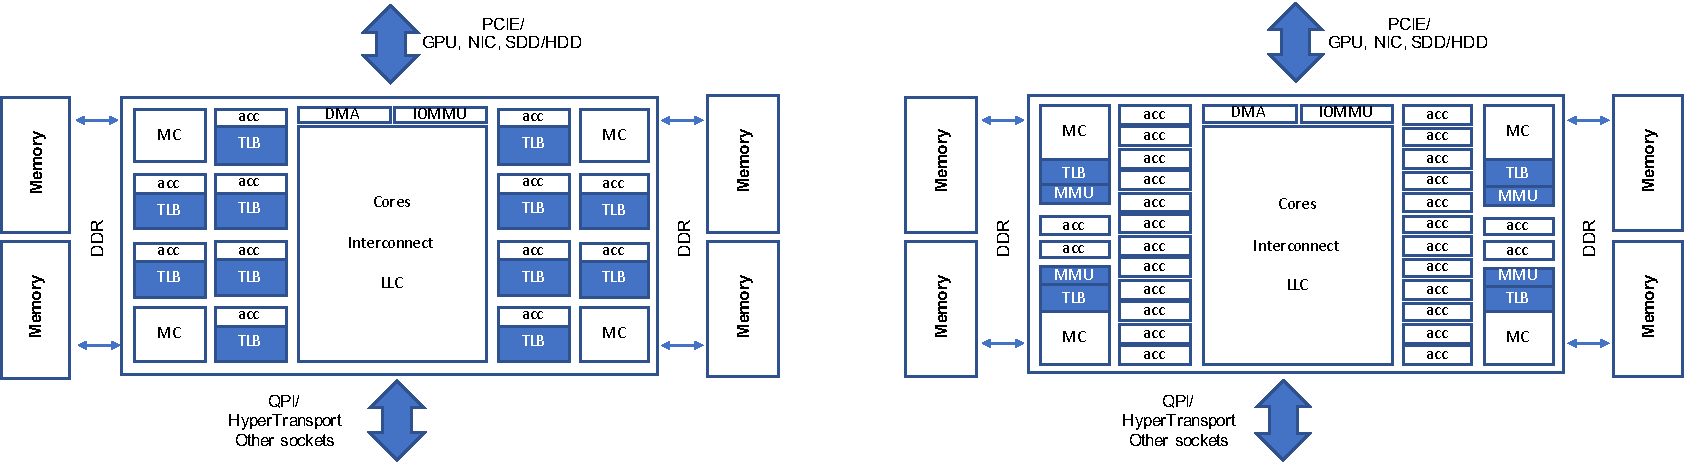
\includegraphics[width=1\textwidth,clip]{figures/overview.pdf}
 \caption{Overview of conventional (left) and DTRIM system (right).}
\label{fig:overview}
\end{figure*}

As the computing industry embraces hardware specialization, research
questions pertaining to the system integration of accelerators are
becoming increasingly important. One such question is that of how to
expose the VM abstraction to accelerators. While initial solutions
allow accelerators to have direct physical access to memory, the
consequent lack of protection, isolation and paging significantly
complicates the software stack. More recent studies have argued that
the conventional VM abstraction and a global address space programming
model is best for software development, enabling "a pointer is a
pointer everywhere" semantics~\cite{pichai:architectural,
  power:supporting, haria:devirtualizing, vesely:observation,
  ausavarungnirun:mosaic}, extending memory protection to
accelerators, and obviating the need for manual inter-CPU-accelerator
data marshalling.

Unfortunately, it is challenging to extend conventional VM to
accelerators in an efficient manner. While general-purpose cores rely
on large hiearchical TLBs to achieve satisfactory VM performance, such
large structures are ill-suited to resource-constrained
accelerators. This is true for a wide spectrum of accelerators ranging
from programmable GPGPUs \cite{pichai:architectural, power:supporting}
to graph processing hardware \cite{haria:devirtualizing} to even more
area-contrained processing in/near memory techniques
\cite{picorel:near-memory}. Furthermore, most accelerators rely on a centralized 
IOMMU for page walks, whose physical distance from the accelerator and from the increasingly 
large and distributed memory makes multi-level page-table walks increasingly slow and inefficient. 


In response, recent studies propose changes to conventional TLB
hardware and the memory allocation/management stack for efficient
address translation and page management on accelerators
\cite{pichai:architectural, power:supporting,
  ausavarungnirun:mosaic}. Among the most promising techniques are
those that obviate the need for large TLBs by relying on translation
contiguity, i.e., situations where large contiguous ranges of virtual
pages are mapped to a corresponding range of spatially-adjacent
physical pages. Contiguous translations can be compressed or coalesced
by TLBs into individual entries, reducing address translation
pressure. While some of these techniques rely on translation
contiguity that OSes may serendipitously generate \cite{pham:colt,
  bhattacharjee:large-reach, cox:efficient, pham:increasing}, the most
successful ones are those that rely on changes to the OS's memory
allocation path so that it produces vast swaths of translation
contiguity \cite{haria:devirtualizing}. Unfortunately, these
techniques, along with similar ones proposed for CPUs
\cite{basu:efficient, gandhi:range}, sacrifice OS flexibility to
generate translation contiguity by requiring, for example, identity
mapping where virtual and physical addresses must be identical (which
can be difficult to achieve in real-world cloud settings where many
applications utilize a machine), or at-allocation contiguity
generation (which can be difficult to achieve in real-world systems
with fragmented memory). %For all these reasons, these techniques have
%the option of falling back on traditional paging.

In contrast, we observe that traditional VM requires large
TLBs because it is {\it fully-associative}; i.e., a virtual page can
map to any physical frame, without restrictions. On the other hand, techniques that cut TLB
requirements by creating massive translation contiguity
\cite{basu:efficient, gandhi:range, haria:devirtualizing} impose
strong restrictions on which physical frames to assign to a virtual
page, reminiscent of the notion of {\it direct-mapping}. Our approach
is to find the sweet spot between these techniques and propose {\it
  set-associative} VM, where a virtual page can map to one among a set
of page frames. We dub this approach DTRIM (Divide \& Translate In Memory). 

DTRIM {\it slightly} restricts VM associativity so that a virtual
address uniquely identifies the region of the physical address space
(a memory chip or partition of arbitrary size) that holds the data. Once the target
memory region is identified, DTRIM performs translation on the memory
side, using local per-region TLBs situated next the corresponding
memory region. In doing so, DTRIM solves two key problems. First, it
facilitates area-efficient TLBs with high hit rates because separate
TLBs are responsible for disjoint parts of the physical address space,
reducing their reach requirements. Second, it dramatically cuts miss
penalties by co-locating translation and data in TLB's physical
partition and performing localized page walks, effectively overlapping 
translation with data fetch. We also show that
the OS support necessary to achieve this approach is compatible with
existing kernels and does not sacrifice flexibility in the mould of
prior work \cite{basu:efficient, haria:devirtualizing}. To showcase
DTRIM's effectiveness, we contribute the following:

\noindent $\bullet$ A study of the VM associativity needs of modern
server workloads. We are inspired by previous work on caches, which
shows how associativity affects capacity, conflict, and compulsory
misses \cite{hill:case}. We find that full VM associativity is often
unnecessary, as most misses---page faults---are either compulsory or
capacity, and are hence insensitive to associativity. 

\noindent $\bullet$ We develop a working prototype of DTRIM by
integrating support for set-associative VM in stock Linux, and show
that these changes are readily implementable. Moreover, we selectively
apply set associativity to {\it regions} of the virtual address space
that benefit from this approach. In so doing, we leave
full-associativity for regions where it is better for performance, and
retain cross-compatibility with existing systems 

\noindent $\bullet$ DTRIM, a translation mechanism which restricts VM
associativity so that a virtual address uniquely identifies a memory
chip/partition, allowing memory accesses to be issued as soon as the
virtual address is known. Each memory partition features an MMU with a
TLB hierarchy, whose location next to the data allows data fetch and
translation to be almost entirely overlapped (for TLB hits and
misses). Each MMU's TLB hierarchy serves only its memory partition,
enabling graceful performance scaling across memory chip/partition
counts.

\noindent $\bullet$ A comparison of DTRIM with well-known translation
mechanisms. DTRIM improves performance by up to $26\%$ and $15\%$ for
in-memory and out-of-memory scenarios respectively, achieving
almost-perfect zero-overhead address translation.
